%!TEX program = lualatex

\documentclass{article}

\usepackage{amsmath}
\usepackage{fontspec}
\usepackage[a4paper, margin=2cm]{geometry}
\usepackage{graphicx}
\usepackage[hidelinks]{hyperref}
\usepackage[cache=false, outputdir=../out]{minted}

\newcommand{\DISCIPLINE}{Бази даних}
\newcommand{\STUDENT}{}
\newcommand{\SUBJECT}{Створення бази даних. Користувачі, ролі, права.}
\newcommand{\TEACHER}{}
\newcommand{\TITLE}{Лабораторна робота №2}
\newcommand{\VARIANT}{33}

\begin{document}

\setmainfont{OpenSans}
\setlength{\emergencystretch}{2cm}

\clearpage\begin{titlepage}
	\begin{center}
		\Large
		Міністерство освіти і науки України \\
		Національний технічний університет України \\
		«Київський політехнічний інститут імені Ігоря Сікорського» \\
		[1\baselineskip]
		Факультет інформатики та обчислювальної техніки \\
		Кафедра інформатики та програмної інженерії \\
	\end{center}

	\vfill

	\begin{center}
		\Large
		\textbf{\TITLE} \\
		з дисципліни \textbf{«\DISCIPLINE»} \\
		на тему: «\SUBJECT»
	\end{center}

	\vfill

	\begin{center}
		\large
		\textbf{Виконав} \hfill \noindent \hrulefill \STUDENT \hrulefill \\
		\small (шифр, прізвище, ім'я, по батькові) \\
		[1\baselineskip]
		\large
		\textbf{Перевірив} \hfill \noindent \hrulefill \TEACHER \hrulefill \\
		\small (прізвище, ім'я, по батькові) \\
	\end{center}

	\vfill

	\begin{center}
		\Large
		Київ \the\year{}
	\end{center}
\end{titlepage}


\clearpage\tableofcontents

\clearpage\section{Мета}

Отримання навичок моделювання предметної області та побудови ER-моделі
предметної області (діаграм "Сутність-Зв'язок").

\section{Робота рієлторської компанії}

У рієлторську компанію звертаються клієнти, які бажають продати/купити чи зняти/здати нерухомість
у оренду. Компанія визначає рієлтора, який буде вести справи клієнтів, на підставі поточної
завантаженості працівників. Виділений рієлтор реєструє клієнта, його контактні дані, тип та
адресу нерухомості, вартість та інші характеристики, а також статус (здача в оренду, продаж,
здача в оренду або продаж). Склад і кількість характеристик може змінюватись відповідно до типу
нерухомості. При виникненні запиту на нерухомість рієлтор зв'язується з клієнтами і погоджує
зручний час і дату огляду нерухомості.

У разі згоди потенційного орендаря на оренду чи покупця на покупку нерухомості рієлтор зв'язується
з ним і погоджує дату оформлення договору про оренду чи покупку. Для здійснення угоди рієлтор оформляє
необхідні дозволи, документи, контракти та договори, після чого передає їх у центральний апарат
компанії для кінцевого нотаріального засвідчення. Вартість послуг рієлтора складає або половину
місячної вартості оренди нерухомості у випадку здачі в оренду, або 2\% від суми угоди при продажі нерухомості.

Клієнти можуть публікувати власні оголошення на оренду чи продаж, але вони публікуються тільки після
проходження модерації адміністратором. В кінці кожного місяця формується звіт про надані рієлторські
послуги та загальний прибуток по кожному типу нерухомості. За результатами аналізу звіту центральний
апарат компанії приймає рішення щодо розширення або звуження штату працівників. Пошуком пропозицій
на здачу в оренду чи продаж нерухомості також займається центральний апарат фірми.

\section{Постановка задачі}

\begin{enumerate}
      \item Вивчити основні теоретичні засади проектування баз даних, семантичного моделювання,
            побудови ER-діаграм (моделей "сутність-зв'язок")
      \item Виділити основні множини сутностей, їх атрибути, зв'язки між ними згідно наданого опису
            предметної області. Мінімальна кількість сутностей - 6.
      \item Побудувати ER-модель предметної області.
      \item За бажанням декомпозувати зв'язки "багато-до-багатьох".
\end{enumerate}

\clearpage\section{ER-діаграма}

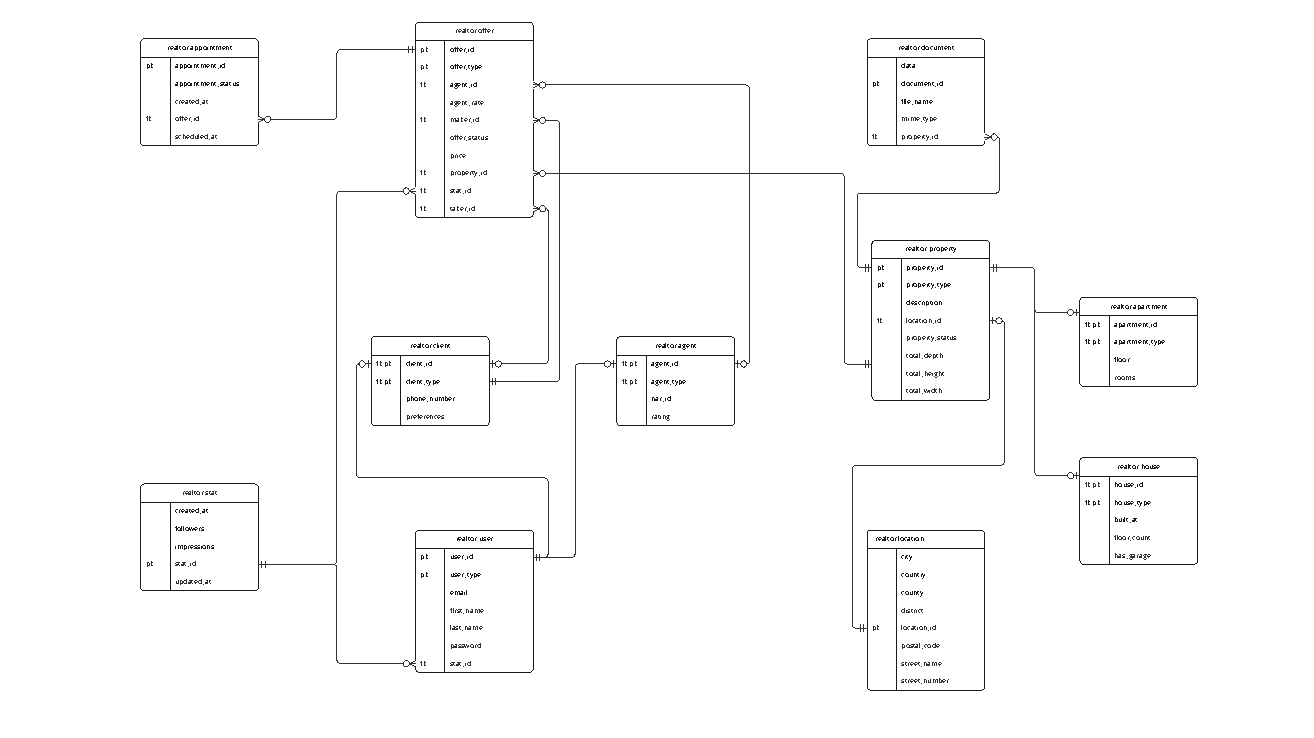
\includegraphics[width=1\linewidth]{../assets/er.pdf}

\section{Зв'язки}

\clearpage\section{Імпортування даних}

PostgreSQL має вбудовані засоби для збереження та відновлення даних.

\begin{enumerate}
	\item pg\_dump - утиліта для створення резервних копій бази даних PostgreSQL.
	      Вона створює надійні резервні копії, навіть якщо база даних використовується одночасно.
	      pg\_dump не блокує доступ інших користувачів до бази даних (читачів або записувачів).
	\item pg\_restore - утиліта для відновлення бази даних PostgreSQL з архіву, створеного pg\_dump.
	      Вона видасть команди, необхідні для реконструкції бази даних до стану, в якому вона була
	      на момент збереження.
\end{enumerate}

За замовчуванням pg\_dump генерує SQL-скрипт. Однак, щоб зменшити обсяг даних, що генеруються,
ви можете вказати параметр "--format=custom" для використання двійкового формату виводу зі стисненням.

\clearpage\section{Код програми}

\inputminted[breakanywhere, breaklines]{yaml}{../docker/compose.yml}
\begin{minted}[breakanywhere, breaklines]{shell}
$ docker compose --file "./docker/compose.yml" up
\end{minted}

\inputminted[breakanywhere, breaklines]{sql}{../sql/00-initdb.sql}
\inputminted[breakanywhere, breaklines]{sql}{../sql/01-faker.sql}
\inputminted[breakanywhere, breaklines]{shell}{../sql/02-dump.sh.log}
\inputminted[breakanywhere, breaklines]{shell}{../sql/03-roles.sh.log}


\end{document}
